\begin{exercice*}[Engrenages]
    \newcommand{\roue}[4]{% #1 = rayon, #2 = nombre de dents, #3 = X centre, #4 = Y centre
        \foreach \i in {1,2,...,#2}
        {
        \pgfmathparse{360*(\i-1)/#2}\let\angle\pgfmathresult

        \begin{scope}[shift={(#3,#4)}]
        \pgfmathparse{#1*cos(90+360/(#2*4))}\let\Ax\pgfmathresult 
        \pgfmathparse{#1*sin(90+360/(#2*4))}\let\Ay\pgfmathresult

        \pgfmathparse{#1*cos(90-360/(#2*4))}\let\Bx\pgfmathresult
        \pgfmathparse{#1*sin(90-360/(#2*4))}\let\By\pgfmathresult

        \pgfmathparse{4*#1*cos(90+360/(#2*8))/3}\let\Cx\pgfmathresult
        \pgfmathparse{4*#1*sin(90+360/(#2*8))/3}\let\Cy\pgfmathresult

        \pgfmathparse{4*#1*cos(90-360/(#2*8))/3}\let\Dx\pgfmathresult
        \pgfmathparse{4*#1*sin(90-360/(#2*8))/3}\let\Dy\pgfmathresult

        \pgfmathparse{90-360/(#2*4)}\let\a\pgfmathresult
        \pgfmathparse{90-1.5*360/(#2*2)}\let\b\pgfmathresult

        \draw[rotate=\angle] (\Ax,\Ay) to[bend left=15] (\Cx,\Cy) -- (\Dx,\Dy) to[bend left=15] (\Bx,\By) arc (\a:\b:#1cm); 
        
        \end{scope}
        }
    }
    % \begin{minipage}{0.6\linewidth}
        On s'intéresse aux engrenages de deux roues.

        Sur la figure ci-dessous les nombres de dents ne correspondent pas à ceux des questions.

        On fait tourner la roue n°$1$ d'un nombre entier de tours.
    % \end{minipage}
    % \begin{minipage}{0.4\linewidth}
        % \hspace*{10mm}
        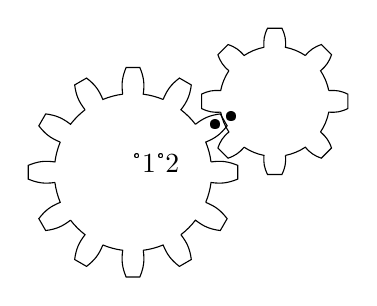
\begin{tikzpicture}
            \roue{1}{12}{0}{0}
            \roue{0.7}{8}{1.8}{0.9}
            \node at (1.05,0.6) {\textbullet};
            \node at (1.25,0.7) {\textbullet};
            \tkzDefPoint(0,0){A}
            \tkzLabelPoint[above](A){roue n°$1$}
            \tkzDefPoint(1.8,0.9){B}
            \tkzLabelPoint[above](B){roue n°$2$}
        \end{tikzpicture}
    % \end{minipage}
    \begin{enumerate}
        \item     La roue n°$1$ possède $6$ dents et la roue n°$2$ a $20$ dents.
        \begin{enumerate}
            \item Écrire la liste des multiples de $6$ et de $20$ jusqu'à trouver un multiple commun.
            \item En déduire le nombre de tours de chaque roue avant le retour à leur position initiale.
        \end{enumerate}
        \item La roue n°$1$ possède $72$ dents et la roue n°$2$ a $39$ dents.
        \begin{enumerate}
            \item Décomposer $72$ et $39$ en produit de facteurs 
            
            premiers.
            \item En déduire le nombre de tours de chaque roue avant le retour à leur position initiale.
        \end{enumerate}
        \item La roue n°$2$ a maintenant $38$ dents. Déterminer le nombre de dents de la roue n°$1$ qui ferait $19$ tours pendant que la roue n°$2$ en fait $8$.
    \end{enumerate}        
    \hrefMathalea{https://coopmaths.fr/mathalea.html?ex=3A12,s=false,n=4&v=l}
\end{exercice*}
\begin{corrige}
    %\setcounter{partie}{0} % Pour s'assurer que le compteur de \partie est à zéro dans les corrigés
    % \phantom{rrr}    \begin{enumerate}
        \begin{enumerate}
            \item 
            \begin{enumerate}
                \item Liste des premiers multiples de $6$ : \\
                $1\times6 = 6$ ; $2\times6 = 12$ ; $3\times6 = 18$ ; $4\times6 = 24$ ; $5\times6 = 30$ ; \\
                $6\times6 = 36$ ; $7\times6 = 42$ ; $8\times6 = 48$ ; $9\times6 = 54$ ; $10\times6 = \mathbf{{\color[HTML]{f15929}60}}$ ; \\
                $11\times6 = 66$ ; $12\times6 = 72$ ; $13\times6 = 78$ ; $14\times6 = 84$ ; $15\times6 = 90$ ; \\
                \dots \\
                Liste des premiers multiples de $20$ : \\
                $1\times20 = 20$ ; $2\times20 = 40$ ; $3\times20 = \mathbf{{\color[HTML]{f15929}60}}$ ; $4\times20 = 80$ ; $5\times20 = 100$ ; \\      
                \dots \\
                \medskip
                \item Le plus petit multiple commun à $6$ et $20$ vaut donc $60$.\\
                Il suffit donc que chaque roue tourne de $60$ dents pour faire un nombre entier de tours et ainsi revenir dans sa position initiale.\\
                En effet, chaque roue doit tourner de façon à ce que le nombre total de dents utilisé soit un multiple de son nombre
                de dents soit au minimum de $60$ dents.\\
                 Cela correspond à $(60\text{ dents})\div (6\text{ dents/tour}) = 10$ tours pour la roue n°$1$.\\
                Cela correspond à $(60\text{ dents})\div (20\text{ dents/tour}) = 3$ tours pour la roue n°$2$.
            \end{enumerate}
            \item Pour un nombre de dents plus élevé, il est plus commode d'utiliser les décompositions en produit de facteurs premiers.\\
            \begin{enumerate}
                \item Décomposition de $72$ en produit de facteurs premiers :  $72 = 2\times2\times2\times3\times3$.\\
                Décomposition de $39$ en produit de facteurs premiers :  $39 = 3\times13$.
               \medskip
                \item Pour retrouver la position initiale,
                chaque roue doit tourner de façon à ce que le nombre total de dents utilisé soit un multiple de son nombre
                de dents.\\
                Soit, grâce aux décompositions précédentes, au minimum de $2\times2\times2\times3\times3\times13 = 936$ dents.\\
                 Cela correspond à $(936\text{ dents})\div (72\text{ dents/tour}) = 13$ tours pour la roue n°$1$.\\
                Cela correspond à $(936\text{ dents})\div (39\text{ dents/tour}) = 24$ tours pour la roue n°$2$.
            \end{enumerate}
            \item Puisque la roue n°$2$, qui a $38$ dents, fait $8$  tours , cela représente $304$ dents.\\
            La roue n°$1$ doit donc aussi tourner de $304$ dents, ceci en $19$  tours .\\
            On obtient donc $(304\text{ dents})\div (19\text{ tours }) = 16 \text{ dents/tour}.$\\
            La roue n°$1$ a donc $16$ dents.
        \end{enumerate}
\end{corrige}

